\section{Results}
\label{sec:results}

\subsection{RQ1: Learning-Curve Quality}

Table~\ref{tab:al-main} reports performance integrated across the full training
budget. $U+H$ obtained the highest mean ROC-AULC (0.933026) and AP-AULC
(0.883336). Relative to Random, its paired fold differences were +0.004249 in
ROC-AULC and +0.014985 in AP-AULC, with the same favorable direction in all five
outer folds. The gains over Uncertainty were smaller: +0.001754 ROC-AULC and
+0.001401 AP-AULC, favorable in four of five folds.

\begin{table*}[t]
\centering
\caption{Active-learning performance, target attainment, and computation. AULC integrates the trajectory over 200--1,200 training labels. Labels-to-target excludes validation labels and the full-pool reference cost.}
\label{tab:al-main}
\small
\setlength{\tabcolsep}{6pt}
\begin{tabular}{lccccc}
\toprule
Policy & ROC-AULC & AP-AULC & Labels to target & Query, 10 rounds (s) & Model + query (s) \\
\midrule
Random & 0.928777 & 0.868350 & 584 & 0.0194 & 4.1947 \\
Uncertainty & 0.931272 & 0.881934 & 520 & 0.0191 & 4.1454 \\
$U+H$ & \textbf{0.933026} & \textbf{0.883336} & 508 & 0.2459 & 4.4741 \\
$U+V$ & 0.930377 & 0.880164 & \textbf{488} & 0.2298 & 4.3826 \\
\xfull & 0.932202 & 0.881638 & 492 & 0.2358 & 4.3471 \\
\bottomrule
\end{tabular}
\end{table*}

$U+V$ did not lead AULC, but it reached the validation target with the smallest
mean training budget, 488 labels. $\xfull$ reached the target at 492 labels. The
latter required 92 fewer labels than Random, a 15.8\% reduction under this target
definition, and 28 fewer than Uncertainty. $U+H$ required 76 fewer labels than
Random (13.0\%). These are oracle-query counts under retained labels; validation
labels and full-pool reference training are additional resources.

The three explanation-guided variants therefore express different trade-offs.
$U+H$ produces the strongest average learning trajectory, $U+V$ reaches the
declared target earliest, and $\xfull$ balances the signals without leading every
criterion. Figure~\ref{fig:al-summary} visualizes this separation. The finding
answers RQ1 positively relative to random acquisition, but only conditionally
relative to uncertainty sampling.

\begin{figure*}[t]
\centering
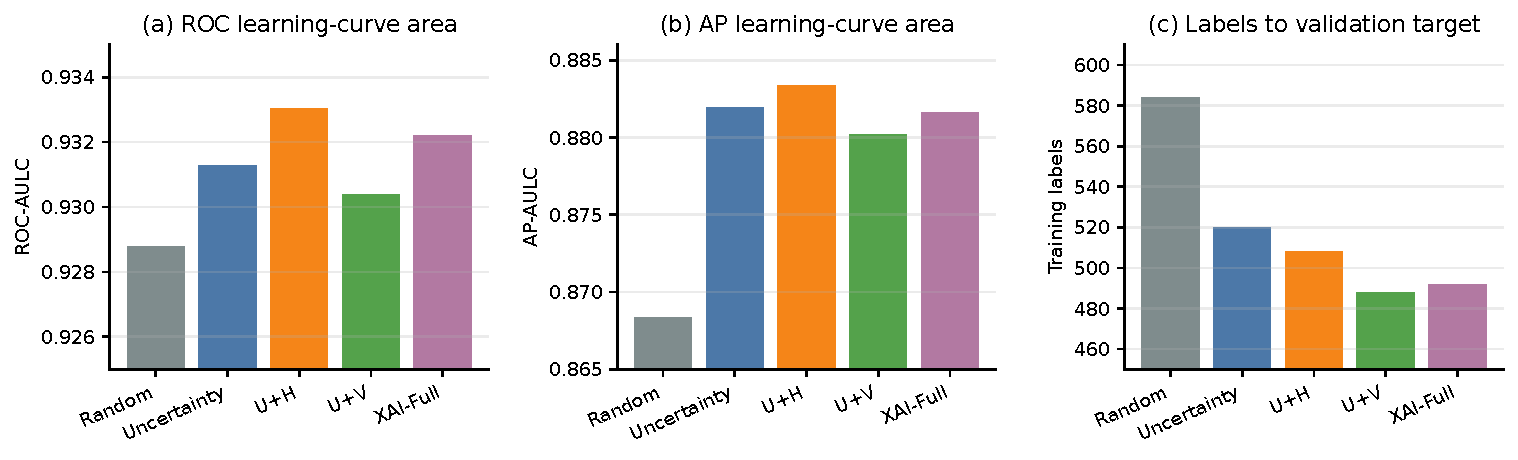
\includegraphics[width=0.93\textwidth]{al_summary.pdf}
\caption{Confirmatory active-learning summaries. Higher AULC is better; fewer
training labels to the predeclared validation target are better. Error bars are
omitted because the readiness snapshot supplies aggregate means and paired fold
effects rather than the underlying fold-level vectors in this checkout.}
\label{fig:al-summary}
\end{figure*}

\begin{table}[t]
\centering
\caption{Selected paired outer-fold effects.}
\label{tab:paired-effects}
\scriptsize
\setlength{\tabcolsep}{2.5pt}
\begin{tabular}{lrrc}
\toprule
Comparison & $\Delta$ROC & $\Delta$AP & Folds \\
\midrule
$U+H$ vs. Random & +0.004249 & +0.014985 & 5/5 \\
$U+H$ vs. Uncertainty & +0.001754 & +0.001401 & 4/5 \\
\xfull vs. Random & +0.003425 & +0.013287 & 5/5 \\
\xfull vs. Uncertainty & +0.000931 & $-0.000297$ & 3/5 \\
\bottomrule
\end{tabular}
\end{table}

Table~\ref{tab:paired-effects} makes the strongest limitation explicit.
$\xfull$ improved ROC-AULC only in three of five fold comparisons against
Uncertainty, and its mean AP-AULC difference was slightly negative. The
three-signal combination is thus not an empirically universal winner. The clearest
evidence for explanation-derived acquisition comes from $U+H$ relative to Random
and, more modestly, relative to Uncertainty.

\subsection{RQ2: Low-FPR Behavior and Computation}

Table~\ref{tab:low-fpr} reports normalized partial-AUC and TPR learning-curve
summaries. All explanation-guided methods improve substantially over Random.
Against Uncertainty, however, differences are small and change sign. Uncertainty
has the highest pAUC at FPR$\leq5\%$ and TPR-AULC at the 1\% cap; $\xfull$ is
highest at the 5\% cap. $U+H$ is slightly below Uncertainty at the 1\% cap and
slightly above it at 5\%.

\begin{table*}[t]
\centering
\caption{Learning-curve summaries in restricted false-positive regions. These are not deployment estimates at FPR $10^{-3}$ or below.}
\label{tab:low-fpr}
\small
\begin{tabular}{lccc}
\toprule
Policy & pAUC, FPR$\leq5\%$ & TPR-AULC, FPR cap 1\% & TPR-AULC, FPR cap 5\% \\
\midrule
Random & 0.804096 & 0.580620 & 0.731980 \\
Uncertainty & \textbf{0.826300} & \textbf{0.638180} & 0.769260 \\
$U+H$ & 0.824774 & 0.636780 & 0.770620 \\
$U+V$ & 0.825194 & 0.626260 & 0.768140 \\
\xfull & 0.823525 & 0.631860 & \textbf{0.771460} \\
\bottomrule
\end{tabular}
\end{table*}

The operating-region result changes the practical interpretation. Explanation
signals improve sample efficiency relative to random annotation, but the retained
study does not establish lower alert burden than a well-implemented uncertainty
baseline. Each outer test fold contains only about 300 benign samples. One false
positive therefore changes FPR by roughly 0.33 percentage points, making much
lower operational regions unresolvable.

Explanation scoring increases computation. $U+H$ adds approximately 0.227~s of
query processing across ten rounds relative to Uncertainty and increases total
model-plus-query time by 7.93\%. $\xfull$ increases the total by 4.86\%; query
processing constitutes about 5.42\% of its reported model-plus-query time. These
small absolute values apply to a 2,000-sample experiment and exclude annotation,
data loading outside the timed scope, and endpoint detection latency.

RQ2 therefore has no single optimal policy. $U+H$ is preferred when integrated
ranking quality is primary, $U+V$ when target attainment under the measured rule
is primary, and Uncertainty remains competitive in the low-FPR summaries while
avoiding TreeSHAP overhead.

\subsection{RQ3: Controlled Deletion}

Table~\ref{tab:deletion} reports AUC decreases averaged over the retained fidelity
models. Under both replacement baselines, top-$|\mathrm{SHAP}|$ deletion has a
large, monotonic effect as $k$ increases, whereas uniform random deletion has a
near-zero mean effect. For mean replacement, the top-minus-random difference is
0.047617 at $k=10$, 0.135323 at $k=25$, and 0.305750 at $k=50$. Median
replacement yields comparable differences of 0.053388, 0.124854, and 0.300119.

\begin{table*}[t]
\centering
\caption{Controlled feature-space deletion across 25 fitted models. Values are ROC--AUC decreases from the corresponding unmasked model.}
\label{tab:deletion}
\small
\begin{tabular}{lrrrr}
\toprule
Replacement & $k$ & Top-SHAP drop & Random drop & Top minus random \\
\midrule
Mean & 10 & 0.047817 & 0.000200 & 0.047617 \\
Mean & 25 & 0.135853 & 0.000530 & 0.135323 \\
Mean & 50 & 0.306729 & 0.000979 & 0.305750 \\
Median & 10 & 0.053483 & 0.000094 & 0.053388 \\
Median & 25 & 0.125180 & 0.000326 & 0.124854 \\
Median & 50 & 0.300777 & 0.000658 & 0.300119 \\
\bottomrule
\end{tabular}
\end{table*}

\begin{figure}[t]
\centering
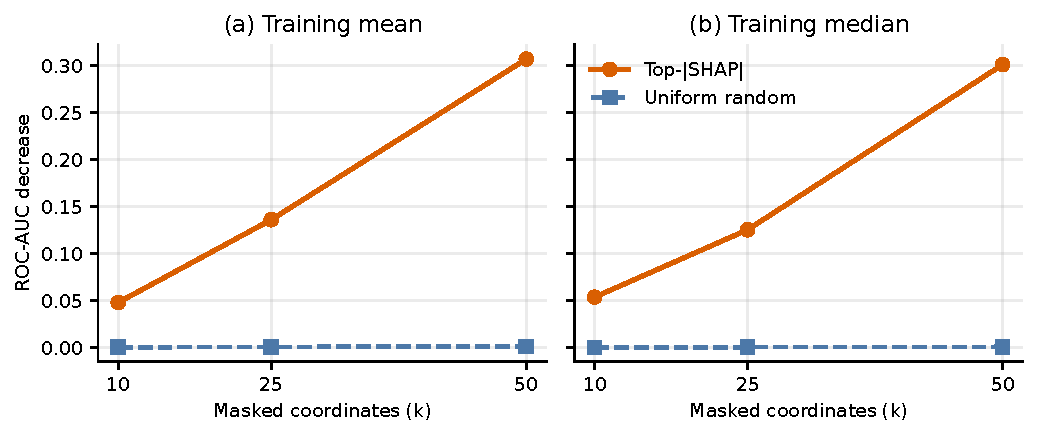
\includegraphics[width=\linewidth]{fidelity_deletion_confirmatory.pdf}
\caption{ROC--AUC decrease under top-$|\mathrm{SHAP}|$ and uniform random
replacement. Absolute effects are emphasized because ratios are unstable when
the random-control decrease is near zero.}
\label{fig:deletion}
\end{figure}

Figure~\ref{fig:deletion} shows that the result is not specific to mean
replacement. It establishes relative fitted-model reliance under both tested
training-derived baselines. Equal coordinate count does not match perturbation
magnitude or ensure that random coordinates participate in the trees; the result
should therefore not be called an executable-level fidelity certificate.

\subsection{RQ3: Attribution-Rank Stability}

Table~\ref{tab:stability} separates model-seed and fold changes. Within a fixed
fold, global Spearman agreement is 0.6144; top-10 Jaccard agreement is 0.6221 and
decreases to 0.4901 at top 50. Across folds, Spearman agreement falls to 0.5512,
and top-k Jaccard values range from 0.4416 to about 0.30.

\begin{table}[t]
\centering
\caption{TreeSHAP ranking stability.}
\label{tab:stability}
\scriptsize
\begin{tabular}{lrrrr}
\toprule
Comparison & $\rho$ & $J_{10}$ & $J_{25}$ & $J_{50}$ \\
\midrule
Seed, same fold & 0.6144 & 0.6221 & 0.5398 & 0.4901 \\
Different fold & 0.5512 & 0.4416 & 0.3073 & 0.3020 \\
\bottomrule
\end{tabular}
\end{table}

\begin{figure}[t]
\centering
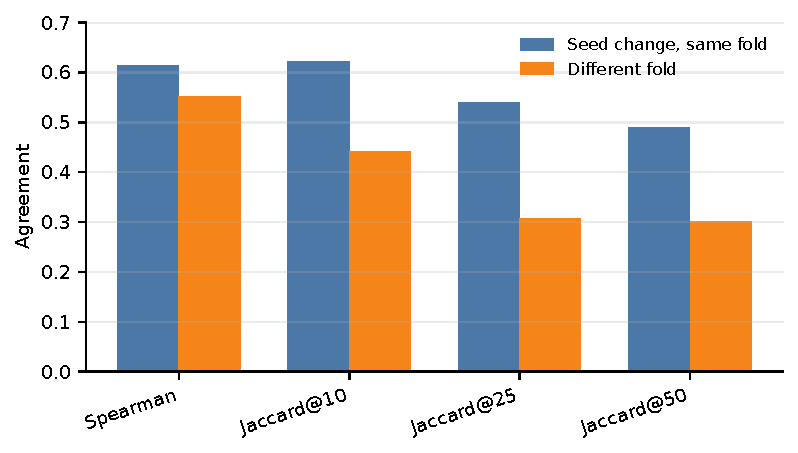
\includegraphics[width=\linewidth]{shap_stability_confirmatory.pdf}
\caption{Global and top-k agreement. Fold changes alter the learned attribution
ranking more than seed changes within a fixed fold.}
\label{fig:stability}
\end{figure}

The rankings are neither arbitrary nor invariant. They exhibit moderate
agreement, with data partitioning exerting more influence than controlled model
randomness. This finding is important for use in acquisition: a sample's
explanation-derived score follows the current fitted model and data partition,
not a stable domain truth.

Mean EC was $0.4268\pm0.0363$, and mean CF was
$0.4680\pm0.0465$ over 25 models. Mean maximum TreeSHAP additivity error was
approximately $6.0\times10^{-15}$. We treat EC and CF as descriptive geometry and
additivity as a numerical check; none of them establishes semantic correctness.

